\documentclass{article}

\usepackage{minted}
\usepackage[most]{tcolorbox}
\usepackage{geometry}
\usepackage{enumitem}
\usepackage{hyperref}
\usepackage{hyperref}
\usepackage[parfill]{parskip}
\usepackage{wrapfig}
\usepackage{accsupp}

\geometry{margin=0.8in}
\definecolor{lightgreen}{rgb}{0.56, 0.93, 0.56}
\definecolor{moonstoneblue}{rgb}{0.45, 0.66, 0.76}
\definecolor{magenta}{rgb}{0.8,0.66,0.76}
\begin{document}
\BeginAccSupp{}
\begin{flushright}
Computational Biology ~\\
Tufts University Bio 35 ~\\
Fall 2021 ~\\ ~\\
\end{flushright}
\begin{center}{\textbf{\Large{Spotlight 1: Ami Bhatt}}}\end{center}

\textit{Please note that in general I have taken/adapted the words of our Spotlight subjects from their own websites to describe their work. I have done this in an effort to maintain accuracy in describing their research programs. Please do not copy paste text from their papers/websites in your assignments!}

\begin{wrapfigure}{L}{0.14\textwidth}
\begin{center}
 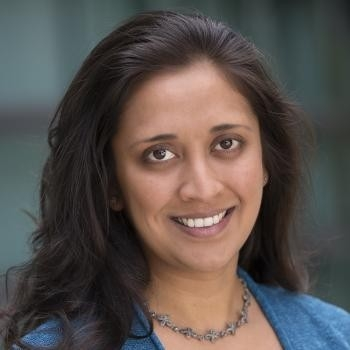
\includegraphics[width=0.13\textwidth]{images/ami-bhatt.jpg}
 \end{center}
\end{wrapfigure}
~\\ As part of our unit on computational gene detection in genomic sequence data, we are going to explore the work of Prof. Ami Bhatt. Amy Bhatt's lab studies the microbiome, the collection of microbes that you might sample from an individual, from the soil, sea water, or another location. Her research group applies modern genetic, molecular and computational techniques to better understand host-microbe interactions and decipher how perturbation of these interactions may result in human disease phenotypes. She is a Professor at Stanford University.

~\\
\vspace{-1em}

Please read the following articles about Ami Bhatt's work on small novel proteins: 
\begin{enumerate}
\item \texttt{\href{https://www.science.org/news/2019/10/new-universe-miniproteins-upending-cell-biology-and-genetics}{https://www.science.org/news/2019/10/new-universe-miniproteins-...}}
\item \texttt{\href{https://www.sciencedirect.com/science/article/pii/S0092867419308384}{https://www.sciencedirect.com/science/article/pii/S0092867419308384}}
\end{enumerate}

\textbf{Optionally}, also listen to the following radio segment:
\begin{enumerate}
\item \texttt{\href{https://player.fm/series/stanford-radio/altering-the-microbiome-with-guest-ami-bhatt}{https://player.fm/series/stanford-radio/altering-the-microbiome-with-guest-ami-bhatt}}
\end{enumerate}

\subsubsection*{Written Assignment} 
After reading the articles about Prof. Bhatt, write a reflection on what you discovered. You might wish to address some of the following: 

\begin{enumerate}
\item What was most interesting to you in reviewing these resources?
\item What did you learn from these resources about computational approaches to finding new genes?
\item What new questions do you have after reviewing these resources?
\item What do these resources tell you about the types of people that do computational biology, or their motivations?
\end{enumerate}

\EndAccSupp{}
\end{document}